\documentclass[Main.tex]{subfiles}

\begin{document}

\begin{multicols}{2}
\begin{flushleft}
\textbf{\textit{\small{По традиции на первых заседаниях научного семинара В . И. Арнольда для студентов Московского университета его участникам предлагается несколько новых задач — точнее, тем для исследования. Среди них иногда встречаются чрезвычайно красивые задачи, формулировки которых понятны даже школьнику. Вот одна из этих тем.}}}
\end{flushleft}

\begin{flushleft}
\huge{\textbf{\textit{МЕАНДРЫ}}} \par
\end{flushleft}

\begin{flushleft}{\small{\textbf{\textit{Академик В. АРНОЛЬД}}}}\end{flushleft}

\noindent Шоссе, идущее с запада на восток, пересекает несколько раз реку, текущую с юго-запада также на восток.
Занумеруем мосты в порядке их следования вдоль шоссе (с запада на восток). Проплывая под мостами вниз по реке, мы будем встречать их, вообще говоря, в другом порядке. Так, например, река на рисунке 1 проходит мосты в порядке 3, 4, 5, 2, 1. Таким образом, эта река определяет перестановку чисел от 1 до 5: (3 4 5 2 1). Ясно, что другая река могла бы протекать иначе и задавать другую перестановку. Но далеко не любая перестановка чисел (мостов) может быть реализована таким образом. (Попробуйте, например, придумать реку, проходящую мосты в порядке 2, 1, 3, 4, 5.) Мы будем называть перестановку \textit{меандром}, если ее можно задать с помощью подходящей реки.

Основной вопрос для нас будет такой: сколько существует различных меандров (т. е. сколько перестановок номеров реализуется), если общее число мостов равно n? Обозначим число \textit{различных меандров с $n$ мостами} через $a(n)$. Легко видеть, что $a(1) = a(2) = 1, a(3) = 2, a(4) = 3$ (рис. 2).

З а д а ч а 1. \textit{Найдите следующие члены последовательности $a(n)$}.

О т в е т : 1, 1, 2, 3, 8, 14, 42, 81, 262, 538, 1828, 3926, 13820, ...

Общая формула для $a(n)$ неизвестна. Неизвестны даже асимптотики $a(n)$ и $a(n + 1)/a(n)$ при $n \rightarrow \infty$.

З а д а ч а 2. \textit{Докажите, что река впервые пересекает шоссе под мостом, номер которого нечетен.}

З а д а ч а 3. \textit{Докажите, что номера 1-го, 3-го, 5-го,... мостов (вдоль реки) нечетны, если нумеровать мосты вдоль шоссе, а номера 2-го, 4-го, ... мостов — четны.}

Начнем классифицировать меандры с того, что зафиксируем первый вдоль реки мост. Обозначим через $a_i(n)$ число меандров с $n$ мостами, для которых река впервые пересекает шоссе под $i$-м (вдоль шоссе) мостом. Согласно задаче 2,

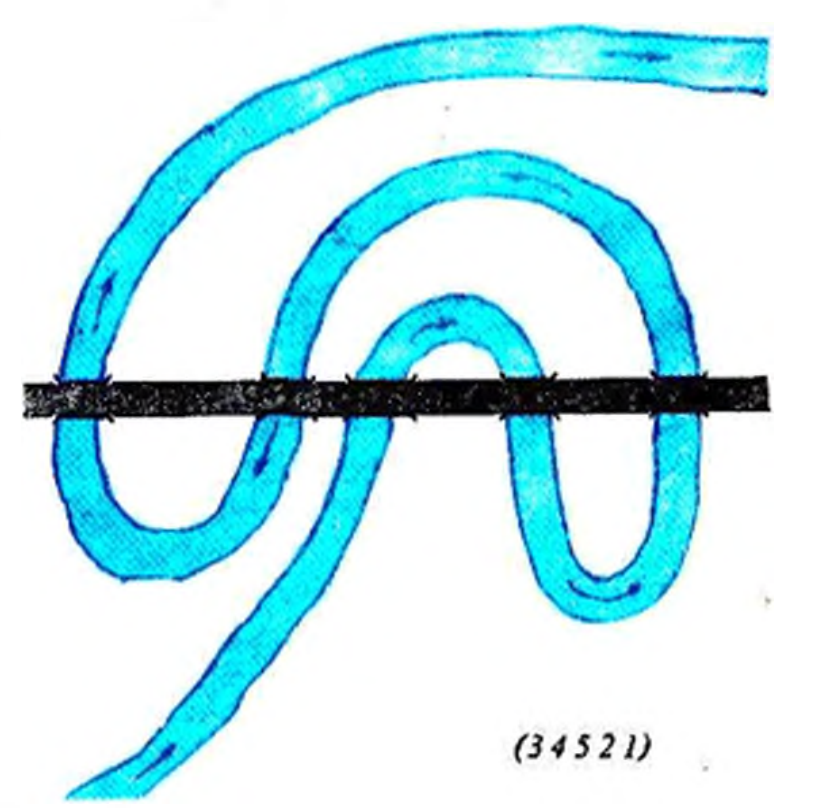
\includegraphics[width=0.5\textwidth]{../images/../images/Picture1}

\begin{flushleft}\textbf{\textit{\small{Рис. 1.}}}\end{flushleft}

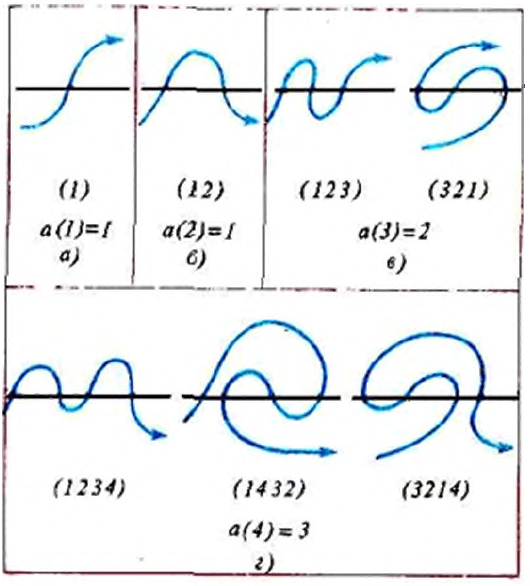
\includegraphics[width=0.5\textwidth]{../images/Picture2}

\begin{flushleft}\textbf{\textit{\small{Рис. 2.}}}\end{flushleft}

\newpage

$$
a(n) = a_1(n) + a_3(n) + ... + a_{2k-1}(n),
$$

\noindent где $n = 2k - 1$ или $n = 2k$.

З а д а ч а 4. Составьте таблицу меандрических чисел $a_i(n)$ при небольших $n$.

О т в е т: для $i,n \leq 10$ см. таблицу.

\begin{center}
\scalebox{0.7}{
\begin{tabular}{ |c|c|c|c|c|c|c|c|c|c|c| } 
\hline
\backslashbox{$a_i(n)$}{$n$} & 1 & 2 & 3 & 4 & 5 & 6 & 7 & 8 & 9 & 10 \\
\hline
    $a(n)$ & 1 & 1 & 2 & 3 & 8 & 14 & 42 & 81 & 262 & 538 \\
    \hline
    $a_1(n)$ & 1 & 1 & 1 & 2 & 3 & 8 & 14 & 42 & 81 & 262 \\
    \hline
    $a_3(n)$ &   &   & 1 & 1 & 2 & 3 & 7 & 14 & 36 & 81   \\
    \hline
    $a_5(n)$ &   &   &   &   & 3 & 3 & 7 & 11 & 28 & 57   \\
    \hline
    $a_7(n)$ &   &   &   &   &   &   & 14 & 14 & 36 & 57   \\
    \hline
    $a_9(n)$ &   &   &   &   &   &   &   &   & 81 & 81   \\
    \hline
    $a_{11}(n)$ &   &   &   &   &   &   &   &   &   &     \\ 
    \hline
    $a_{13}(n)$ &   &   &   &   &   &   &   &   &   &     \\
\hline
\end{tabular}
}
\end{center}

З а д а ч а 5. \textit{Найдите в этой таблице закономерности. Случайно ли число 14 появилось пять раз?}

З а д а ч а 6. \textit{Докажите, что\\
\indent    1) $a(n) = a_1(n+1),$\\
\indent    2) $a_i(n) =  a_j(n)$, если $i + j = n + 1$ четно,\\
\indent    3) $a_i(n) = a_j(n)$, если $i + j = n + 2$ четно, $i \geq 3$, $j \geq 3$,\\
\indent    4) $a_1(2k-1) = a_3(2k)$,\\
\indent    5) $a(2k+1)$ четно.\\
}

З а д а ч а 7. \textit{Четно ли $a(16)$?}

З а д а ч а 8 . \textit{Докажите, что $a(n)$ нечетны только, если $n = 2^i$.}

З а д а ч а 9. \textit{Исследуйте поведение при $k \rightarrow \infty$ распределений $a_i(2k + 1)$, где $i \geq 1$ и $a_i(2k)$, где $i \geq 3$.}

З а д а ч а 10. \textit{Докажите, что всякая перестановка $n$ мостов может быть реализована меандрирующей рекой, если шоссе и река находятся не на плоскости, а на подходящей поверхности, скажем на плоскости с приклеенными к ней ручками (рис. 3).}

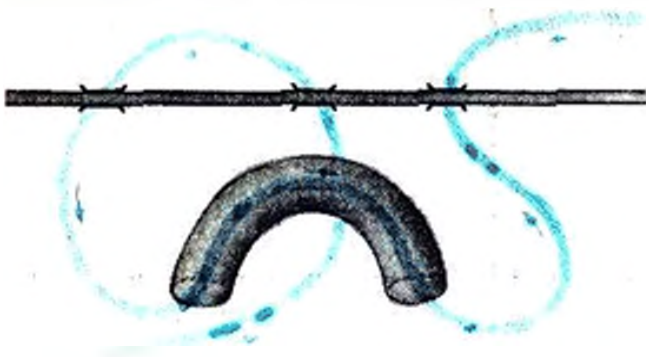
\includegraphics[width=0.4\textwidth]{../images/Picture3}

\begin{flushleft}\textbf{\textit{\small{Рис. 3.}}}\end{flushleft}

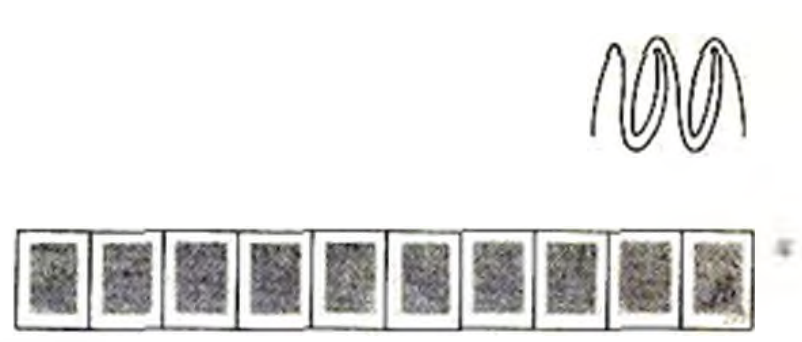
\includegraphics[width=0.4\textwidth]{../images/Picture4}

\begin{flushleft}\textbf{\textit{\small{Рис. 4.}}}\end{flushleft}

Минимальное число ручек такой поверхности назовем родом перестановки. Таким образом, все перестановки распределяются по родам. Обычные меандры — это перестановки рода нуль.

З а д а ч а 11. \textit{Исследуйте распределение перестановок из $n$ элементов по родам при $n \rightarrow \infty$.}

З а д а ч а 12. \textit{Перенесите преды дущие рассмотрения на меандры, образованные нескольким и реками.}

З а м е ч а н и я

1. Число таких обобщенных меандров, образованных системами замкнутых рек, на проективной плоскости при пересечении с бесконечно удаленным шоссе — это известные числа Каталана 1, 1, 2, 5, 14, 42,...

Число Каталана $c(n)$ проще всего определить как число способов расстановки скобок в произведении из $n$ сомножителей. Например, $c(3) = 2$. Два способа расстановки скобок — это $(ab)c$ и $a(bc)$. В произведении четырех сомножителей скобки можно расставить пятью способами:
$$
((ab)c)d, (ab)(cd), (a(bc))d, a((bc)d), a(b(cd)).
$$

\noindent Поэтому $c(4) = 5$  и т.д.

Числа Каталана обладают замечательным свойством неожиданно возникать в самых разных задачах. Подробнее об этом можно узнать из статьи М. Гарднера «Числа Каталана» («Квант», 1978, № 7, с. 20).

2. С задачей о меандрах связана следующая «задача о марках»: сколькими способами можно сложить в стопку ленту, состоящую из $n$ марок (рис. 4; вверху показан один из способов складывания полоски). Об этой задаче рассказано в книге М. Гарднера «Математические досуги» (М.: Мир, 1972, с. 344 — 353).

\begin{center}
    \textbf{\textit{\tiny{(Окончание см. на с. 14)}}}
\end{center}

\end{multicols}

\end{document}
